% apdxa.tex

\chapter{Appendix: How to Add an Appendix}
\label{apdx:a}

This is Appendix~\ref{apdx:a}.

You can have additional appendices too, (\emph{e.g.}, \texttt{apdxb.tex},
\texttt{apdxc.tex}, \emph{etc.}). These files need to be included in
\texttt{thesis.tex}.

If you don't need any appendices, delete the appendix
related lines from \texttt{thesis.tex}.

\begin{figure}
\centering
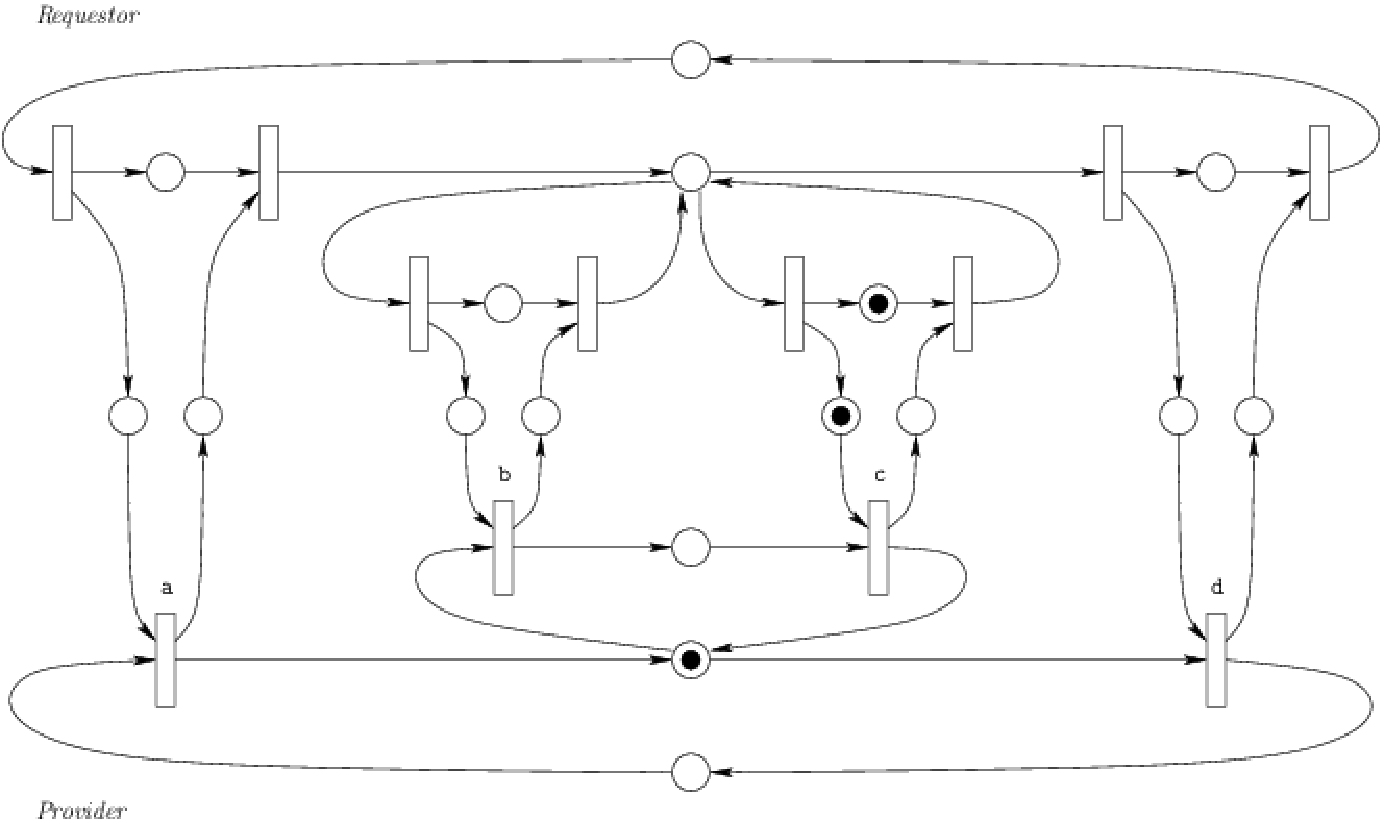
\includegraphics[scale=0.40]{Images/db-deadlock}
\caption{\label{fig:app-db-deadlock} Image of a deadlocked Petri net at 40\%
  scaling.} 
\end{figure}

\begin{table}[!htbp]
\centering
\caption{Fall Semester Enrollment}
\label{tab:app-pop}
\vspace{2mm}
\begin{tabular}{c||c|c|c||c|c|c|}
\hline
	& \multicolumn{3}{c||}{Undergraduate}
	& \multicolumn{3}{c|}{Graduate} \\
\cline{2-7}
     & F/T & P/T & Total & F/T & P/T & Total \\
\cline{2-7}
2004 & 13,191 & 2,223 & 15,414 & 1,308 & 879 & 2,187 \\
2005 & 13,184 & 2,143 & 15,327 & 1,375 & 920 & 2,295 \\
2006 & 12,809 & 2,224 & 15,033 & 1,373 & 899 & 2,272 \\
2007 & 12,634 & 2,155 & 14,789 & 1,403 & 899 & 2,302 \\
2008 & 12,269 & 2,208 & 14,477 & 1,410 &1,005& 2,415 \\
2009 & 12,382 & 2,323 & 14,705 & 1,567 &1,106& 2,673 \\
\hline
\end{tabular}
\end{table}

\section{Equations}
An example mathematical formulae is show in~\ref{eqn:appsum}.

\begin{equation}\label{eqn:appsum}
\sum_{i = 0}^{n} i^2
\end{equation}
